\section{The 2-D Ising Model Concluded, The 3-D Ising Model}
\subsection{Kramers-Wannier Duality}
\subsubsection{High-Temperature Expansion}
Our discussion of the high-$T$ discussion in the 2-D Ising model leads us to the notion of Kramers-Wannier duality (a feature unique to $D = 2$). We will not derive it from scratch, as the derivation is not particularly illuminating. But the plausibility argument for it is quite convincing.

Historically - the solution to the 2D Ising model was very striking. There was Landau theory, which had not been disproven up until this point. But then the 2D Ising model was solved and had different critical exponents to the mean field prediction.

Recall we wrote the partition function in the form:
\begin{equation}
    Z = \left(2\cosh\frac{J}{k_B T}\right)^N\sum_{\text{spins}}\prod_{\text{links}}\left(1 + (\tanh\frac{J}{k_B T})\sigma_x\sigma_{x + i}\right)
\end{equation}

Expanding the product the high-temperature limit (where $\tanh\frac{J}{k_B T}$ is small), we had the zeroth order contribution as just $1$. For the corrections, we needed that each spin $\sigma_x$ needs to appear twice in order for the contribution to be nonvanishing (if the spin only appears once, the term vanishes when we take the sum over spins as the $\pm 1$ appears. But $\sigma_i^2 = 1$ terms contribute); the smallest possible contribution is therefore a square consisting of the 4 spins on the corners (each of which are hit twice). The contribution looks like:
\begin{equation}
    N\left(\tanh\frac{J}{k_B T}\right)^4
\end{equation}
where the $N$ is for the $N$ possible squares, and the $4$ is for the four links that appear in this term.

The next contribution comes from a rectangle 3 spins long and 2 spins wide, so 6 spins in total. The contribution therefore looks like:
\begin{equation}
    2N\left(\tanh\frac{J}{k_B T}\right)^6
\end{equation}

The next contribution comes from 2 squares of 4 spins each. This contribution looks like:
\begin{equation}
    \frac{N(N-4)}{2}\left(\tanh\frac{J}{k_B T}\right)^8
\end{equation}
where the prefactor can be explained as follows. There are $N$ places we can put the first square, and $N-4$ places we can put the second. But then the two squares are indistinguishable (the order of choosing the squares does not matter) so we divide by $2$ to prevent overcounting. 

\begin{figure}[htbp]
    \centering
    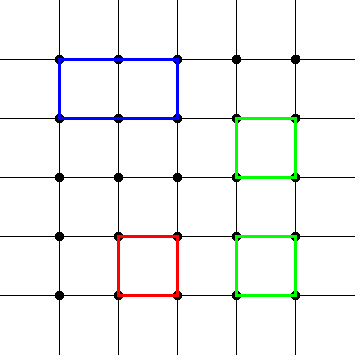
\includegraphics{Images/fig-loops.pdf}
    \caption{Contributions to the high-temperature expansion in the form of closed loops on the lattice. The first contribution comes from 4-site loops (red). The next contribution comes from 6-site loops (blue). The next contribution comes from 8-site loops (green) and so on.}
    \label{fig-loops}
\end{figure}

So, the product can be written as:
\begin{equation}
    \prod_{\text{links}}\left(1 + (\tanh\frac{J}{k_B T})\sigma_x\sigma_{x + i}\right) = 1 + N\left(\tanh\frac{J}{k_B T}\right)^4 + 2N\left(\tanh\frac{J}{k_B T}\right)^6 + \frac{N(N-4)}{2}\left(\tanh\frac{J}{k_B T}\right)^8 + \ldots
\end{equation}
which we can write as:
\begin{equation}
    = e^{N\left(\tanh\frac{J}{k_B T}\right)^4 + N\left(2\left(\tanh\frac{J}{k_B T}\right)^6 - 2\left(\tanh\frac{J}{k_B T}\right)^8\right) + \ldots }
\end{equation}
where we can see the first couple terms that we have discussing come out by Taylor expanding the exponential.

\subsubsection{Low-Temperature Expansion}
In low temperatures, we expect a completely ordered phase, where all of the spins are aligned. Let us choose the all-spin-up state as the leading term. The partition function if we just include the ground state looks like:
\begin{equation}
    Z = e^{2\frac{J}{k_B T}N} + \ldots
\end{equation}
where $-2\frac{J}{k_B T}N$ is the ground state energy, where we have $2N$ aligned links.

How do we correct this? We include excitations. The first correction comes from a single spin being flipped from $+1$ to $-1$. We have 4 bonds flipped, each with energy cost 2, so:
\begin{equation}
    Z = e^{2\frac{J}{k_B T}N}\left(1 + N\left(e^{-\frac{2J}{k_B T}}\right)^4 + \ldots \right)
\end{equation}

\begin{figure}[htbp]
    \centering
    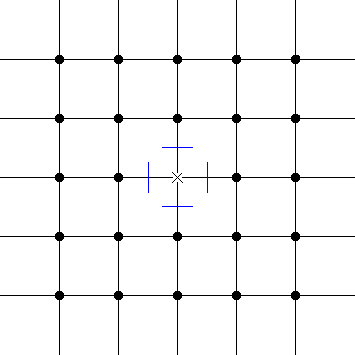
\includegraphics{Images/fig-onespinflip.pdf}

    \caption{A single spin being flipped from $+1$ to $-1$ (denoted by the $\times$) leads to the flipping of 4 bonds (blue) around it.}
    \label{fig-onespinflip}
\end{figure}
But let's think about this geometrically. If we flip one spin at a site on the physical lattice, we can equivalently view this as a loop on the dual lattice. So, we can see the equivalent structure of the high and low temperature expansions. The high temperature expansion is in loops on the physical lattice, and the low temperature expansion is in loops on the dual lattice. This observation is basically what is known as \emph{Kramers-Wannier duality}.

\begin{figure}[htbp]
    \centering
    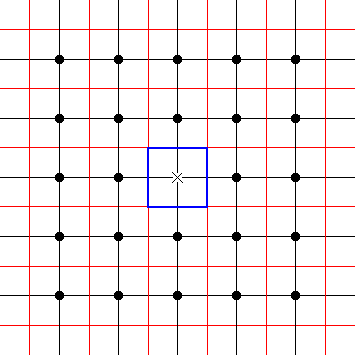
\includegraphics{Images/fig-KWduality.pdf}
    \caption{Visualization of Kramers-Wannier duality for the 2D Ising model. The high temperature expansion can be viewed as an expansion in loops on the physical lattice (black), and the low temperature exapnsion can be viewed as an expansion of loops on the dual lattice (red).}
    \label{fig-KWduality}
\end{figure}

So what we can do is consider Ising models on the original and dual lattices, and then match up the coefficients. If our original Ising model has the factor $e^{-\frac{2J}{k_B T}}$ in the low-$T$ expansion and the dual lattice has the factor $\tanh\frac{\tilde{J}}{k_B T}$, we can then equate:
\begin{equation}
    e^{-\frac{2J}{k_B T}} = \tanh\frac{\tilde{J}}{k_B T}
\end{equation}
what does this duality do for us? it really interchanges the high and low temperature limits. Also, one can argue that the low-$T$ on the original lattice is a magnetized phase, and high-$T$ on the dual lattice is a magnetized phase, so when we have a self-dual we must have that the magnetization is zero, i.e. the critical temperature $T_c$ solves:
\begin{equation}
    e^{-\frac{2J}{k_B T_c}} = \tanh\frac{J}{k_B T_c}
\end{equation}

This Kramers-Wannier duality is quite useful (and special to 2D, though there does exist Dirac duality in 4 spacetime dimensions). We can use it to learn about the system even when things are not self-dual, for example if we know there is a phase transition in the low-$T$ regime we immediately obtain that there is a phase transition in the high-$T$ regime as well.

Also note that there is a quantum analog to this (a gas of non-interacting Majorana fermions).

\subsection{Onsager Exact Solution and Critical Exponents}
Onsager (through some method) found the expression for the free energy to be:
\begin{equation}
    F = -k_B T N \left(2\cosh\frac{J}{k_B T} + \frac{1}{2}\right) + \frac{1}{2\pi^2}\int_0^\pi dp_1 \int_0^\pi dp_2 \ln\left[1 - \frac{\sinh\frac{J}{k_B T}}{\cosh^2\frac{J}{k_B T}}\left(\cos p_1 + \cos p_2\right)\right]
\end{equation}
From this expression we can search for the critical exponents.
\begin{table}[htbp]
    \centering\begin{tabular}{|c|c|c|}
        \hline Exponent & 2-D Ising Model & Mean Field theory
        \\ \hline $\alpha$ & $0$ & $0$
        \\ $\beta$ & $\frac{1}{8}$ & $\frac{1}{2}$
        \\ $\gamma$ & $\frac{7}{4}$ & $1$
        \\ $\delta$ & $15$ & $3$
        \\ $\eta$ & $\frac{1}{4}$ & $\frac{1}{2}$
        \\ $\nu$ & $\frac{1}{2}$ & $0$
        \\ \hline
    \end{tabular}
    \caption{Critical exponents of the 2D Ising model, compared with the critical exponents of mean field theory.}
    \label{table-2dIsingcriticalexponents}
\end{table}
The solutions to the lattice model here are exact. One other interesting development is a model which just looks at the long-wavelength degrees of freedom of the spins. Assuming scale variance, we can solve the theory; scale invariance implies conformal invariance, of which there will be an infinite number of symmetries in 2D, and this can be solved using algebra. The techniques agree, and so studying the long-wavelength behaviour study is promising.

Another comment; does this generalize to higher dimensions? Well, the high-$T$ expansion is not particularly dimension dependent. The low-$T$ expansion is. The dual lattice is really special to 2 dimensions. Let us discuss this - what if we were in 3 dimensions and wanted to do a low temperature expansion? Well, if we flip a single spin on the 3D lattice, we would now have that there are six bonds that are flipped, forming a cube (a volume) around the flipped spin. The high $T$ expansion is in loops, the low $T$ expansion is in surfaces. So, the dual lattice does not resemble an Ising model.

Next lecture - we will begin to look at the Ising model in 3D, and for this we will use renormalization group techniques.